\documentclass[12pt, a4paper]{article}

\usepackage{authblk}
\usepackage[utf8]{inputenc}
\usepackage[T2A]{fontenc}
\usepackage[serbianc]{babel}
\usepackage{hyperref}
\usepackage{amsmath}
\usepackage{graphicx}
\newtheorem{primer}[Пример]{section}

\renewcommand\Authsep{\par}
\renewcommand\Authands{\par}

\title{Увод у каузално (узрочно) закључивање}
\author{Александра Новаковић 368/22}
\author{Милица Ињац 338/18}
\author{Бојан Корда 121/19}
\affil{Математички факултет, Универзитет у Београду}
\date{\today}

\begin{document}
\maketitle
\newpage

\tableofcontents
\newpage

\section{Фундаментални проблем}
\subsection{Увод}
У многим применама статистике, велики део истраживачких питања заправо је питање каузалности, а не само описивања података или испитивања њихове повезаности.
На пример, медицински истраживач може желети да утврди да ли је нови лек заиста ефикасан у лечењу одређене болести. Економиста може бити заинтересован за 
испитивање ефеката програма обуке на запосленост појединаца, док социолог може проучавати како развод родитеља утиче на даљу едукацију деце. 
У свим овим примерима циљ је да се утврди узрочни однос између одређене интервенције и исхода, а не само да се опишу обрасци у подацима.

За разлику од пуке корелације, каузално закључивање тежи да одговори на питање: \textit{„Шта би било, кад би било?“} Ову идеју можемо јасније приказати на примеру из 
филма „Диван живот“, у којем главни лик, Џорџ Бејли, пролази кроз дубоку кризу и тврди да би свет био боље место да се он никада није родио. У том тренутку појављује 
се анђео који му показује како би свет изгледао у контрафактуалном сценарију — свету у којем Џорџ није постојао. У том свету, између осталог, његова деца никада нису 
рођена, његов млађи брат умире као дете јер није било никога да га спаси, а фармацеут погрешно издаје рецепт и бива осуђен за убиство из нехата. Супротстављањем 
стварног света (у којем је Џорџ присутан) и контрафактуалног света (у којем га нема), филм сликовито приказује суштину каузалног закључивања: поређење између онога 
што јесте и онога што би могло да буде.

Идеја каузалног закључивања заснива се на поређењу стварно посматраног исхода са потенцијалним исходима који би се могли догодити да је третман био другачији. 
Међутим, проблем је у томе што те алтернативне исходе никада не можемо посматрати директно — они су контрафактуални. Због тога се каузално закључивање у 
основи може посматрати као проблем са недостајућим подацима: од кључног значаја је механизам који одређује који подаци су посматрани, а који не. У контексту 
каузалне анализе, овај механизам назива се механизам доделе третмана, јер одређује који ентитети добијају који ниво третмана.

Ово поглавље и следеће баве се каузалним закључивањем, које се односи на питање шта би се догодило са неким исходом $y$ као резултат хипотетичког третмана.
У оквиру регресионог модела, третман се може представити променљивом $T$:
$$
T_i =
\begin{cases}
1, & \text{ако јединица} i \text{добије третман},\\
0, & \text{ако јединица} i \text{припада контролној групи}
\end{cases}
$$
а у случају континуираног третмана, $T_i$ представља ниво третмана који је додељен јединици $i$.

У уобичајеном регресионом контексту, предиктивно закључивање се односи на поређења између различитих јединица, док се каузално закључивање бави 
поређењем различитих третмана који би били примењени на исту јединицу. Уопштено посматрано, каузално закључивање се може сматрати посебним случајем предикције, 
у којем је циљ да се предвиди шта би се догодило под различитим опцијама третмана.

Коришћење контролисаних студија представља најефикаснији начин за утврђивање узрочних веза између променљивих. У контролисаној студији, узорак или популација 
се дели на две групе које су међусобно упоредиве по скоро свим карактеристикама. Након тога, групе добијају различите третмане, а њихови исходи се посебно 
анализирају и упоређују.

\subsubsection{корелација не повлачи узрочност}
Каузалност је област статистике која се често погрешно разуме и неправилно примењује због уверења да, ако подаци показују корелацију, 
нужно постоји и узрочна веза иза тога.

Када петао запева, убрзо након тога сунце излази — али знамо да петао није узрок изласка сунца. Да је петла појео сеоски мачак, сунце би ипак свануло.
У једној студији индустрија чоколаде је тврдила да „конзумирање чоколаде производи Нобелове лауреате“. Иако би конзумација чоколаде могла утицати на повећање броја 
Нобелових лауреата, обрнуто је такође могуће — повећање броја лауреата могло је довести до повећане потрошње чоколаде, нпр. због прослава. Вероватније је да 
непосматране променљиве, као што су социо-економски статус или квалитет образовног система, могу истовремено утицати и на потрошњу чоколаде и на број лауреата, чиме 
је корелација између њих неузрочна. 

\begin{figure}[h!]
    \centering
    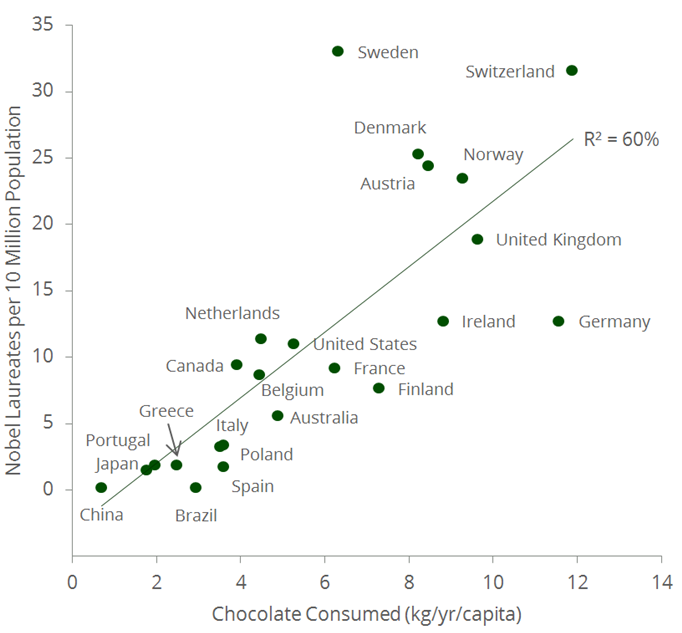
\includegraphics[width=0.7\textwidth]{Chocolate_consumption.png}
    \caption{Конзумација чоколаде и добитници Нобелове награде. Преузето са: \textit{https://www.dectech.co.uk/news-insights/buzz/why-is-correlation-not-causation-part-i/}}
    \label{fig:uzrocnost}
\end{figure}

Да бисмо избегли оваква погрешна тумачења, важно је јасно разграничити шта је корелација, а шта каузалност и разумети на који начин се ови односи испитују у статистици.

Корелација и каузалност представљају две различите врсте односа између променљивих. Корелација описује статистичку повезаност: две променљиве се крећу заједно на 
предвидљив начин, али то не значи да промена једне узрокује промену друге. Каузалност, с друге стране, подразумева да промена једне променљиве директно доводи до 
промене друге, при чему постоји стварна узрочна веза. Док корелација мери само обрасце заједничког кретања података, каузалност захтева разумевање механизма који 
повезује променљиве и обично укључује контролу других фактора који могу утицати на посматрани однос.

Корелација представља најнижи ниво каузалне хијерархије и дефинише се поређењем очекиваног исхода код тренираних и нетретираних у стварном свету, $E[Y|A=1] \neq E[Y|A=0]$.
Каузалност подразумева поређење целокупне популације када би сви били третирани, $E[Y^{a=1}]$, са исходом када би сви били нетретирани, $E[Y^{a=0}]$.
Корелација може постојави чак и када међу њима нема каузалне везе, обично због постојања заједничког узорка.
Принцип заједничког узрока формализује ове могућности: ако су две случајне променљиве $X$ и $Y$ статистички 
зависне, онда је могуће да 
\begin{enumerate}
    \item $X$ узрокује $Y$
    \item $Y$ узрокује $X$
    \item постоји трећа променљива $Z$ која узрокује и $X$ и $Y$, при чему $X$ и $Y$ постају независне ако се узме у обзир $Z$
\end{enumerate}
Каузално закључивање пружа алате који нам омогућавају да донесемо узрочне закључке чак и у одсуству истинског експеримента, под условом да су испуњене
одређене претпоставке (условна заменљивост, позитивност и конзистентност) о којима ће бити речи касније. 

Да би се боље разумела практична важност каузалног закључивања, корисно је погледати како оно функционише у стварним истраживачким ситуацијама и како помаже да се 
избегну погрешни закључци засновани само на корелацији.

\subsubsection{Главне разлике, истраживања, илустрација примером}
Каузално закључивање је важно, на пример, у медицинским истраживањима једна група може добијати плацебо, док друга добија нови тип лека.
Ако се исходи између те две групе значајно разликују, управо различита искуства могу бити узрок тих различитих исхода.

Поред експерименталних дизајна, каузално размишљање је кључно и код анализа опсервационих података. Један од феномена који најбоље илуструје ову потребу јесте 
Симпсонов парадокс.

Симпсонов парадокс представља појаву у којој се однос између две променљиве мења или чак потпуно преокреће када се подаци 
посматрају у целини у односу на њихове подгрупе. Другим речима, корелација која важи на агрегатном нивоу може нестати или 
се обрнути када се подаци разбију по релевантним категоријама.

Овај парадокс јасно показује зашто „корелација не повлачи узрочност“ – наизглед јака веза може бити последица прикривених 
(конфаундирајућих) фактора. %ovde dodati i primer sa doktorima
Класичан пример је анализа успеха лечења код мушкараца и жена: када се посматрају подаци укупно, 
једна терапија делује успешније, док када се подаци раздвоје по полу, испостави се да је друга терапија боља у обе групе.

Суштина Симпсоновог парадокса је у томе да исту корелацију можемо тумачити потпуно другачије у зависности од нивоа анализе. 
Због тога се у каузалном закључивању наглашава важност идентификације и контроле скривених променљивих како би се избегли 
погрешни закључци.

Разликовање корелације и каузалности је само први корак ка разумевању узрочних односа. Да бисмо могли прецизније да објаснимо и измеримо ефекте различитих интервенција, 
потребан нам је формалнији оквир. У наставку ће бити представљени кључни појмови као што су контрафактуални исходи, просечни третмански ефекат (ATE), претпоставка 
SUTVA и Рубинов каузални модел, који нам помажу да каузално размишљање претворимо у конкретне статистичке алате.


\subsection{Фундаментални проблем}
    \subsubsection{Рубинов каузални модел}

Фундаментални проблем каузалног закључивања, како га је назвао Пол Холанд 1986. године, чињеница да за сваку појединачну јединицу (особу, објекат) која је 
предмет истраживања може бити посматран само један од два потенцијална исхода. То значи да не можемо истовремено посматрати шта се дешава са једним појединцем након 
што је примио третман (нпр. $T=1$) и шта се дешава са тим истим појединцем након што није примио третман (нпр. $T=0$), у истом тренутку. Другим речима, каузални ефекат 
на индивидуалном нивоу увек остаје делимично непознат, јер је један од исхода нужно контрафактуалан (непосматран, хипотетички исход, супротан посматраним чињеницама).
Због ове немогућности истовременог посматрања, никада не можемо директно измерити индивидуални каузални ефекат.

Доналд Рубин је 1974. године формализовао овај проблем и увео основни језик за кодирање каузалности. Овај модел назива се Рубинов Каузални Модел (РЦМ), састоји се 
из три градивна блока, кључних за дефинисање каузалног ефекта.
\begin{enumerate}
    \item \textbf{Потенцијални исходи} За сваку јединку $i$, дефинишу се два потенцијална исхода, $Y_i^1$ или $Y_i^0$ у зависности од тога да ли 
    је јединка примила третман ($T_i=1$) или није ($T_i=0$). Пре доношења одлуке о додели третмана, оба ова стања су теоретски изводљива за сваку јединку па се каузални 
    ефекат дефинише као разлика потенцијалних исхода, односно $\Delta^Y_i = Y_i^1 - Y_i^0$.
    \item \textbf{Правило доделе третмана} То је променљива $D_i$ која одлучује ко прима третман ($Т_i=1$) и ко остаје у контролној групи ($Т_i=0$). Правило 
    доделе је кључно јер одређује који од два потенцијална исхода ће бити посматран. Механизам додељивања третмана је важан јер утиче на очекиване вредности потенцијалних исхода.
    \item \textbf{Једначина преклапања, прекидна једначина} Ова једначина повезује посматрани исход $Y_i$ са потенцијалним исходима, преко променљиве $D_i$: $Y_i = D_i Y^1_i + (1 - D_i) Y^0_i$.
    Оне објашњава да посматрамо само исход који одговара третману који је заиста примљен.
\end{enumerate}
РЦМ је, у суштини, модел о делимично посматраним случајним варијаблама па се каузално закључивање може посматрати као предвиђање шта би се догодило са јединицом $i$ 
ако би $D_i=0$ или $D_i=1$.

Да би потенцијални исходи били добро дефинисани, неопходна је претпоставка о стабилној вредности третмана јединице (\textit{eng. Stable Unit Treatment Value Assumption, SUTVA}), 
која подразумева да исход једне јединке не зависи од третмана других и да не постоје скривене варијанте третмана. 
Na primer, ishod jedne osobe koja prima transplantaciju srca ne bi trebalo da zavisi od toga da li je i druga osoba primila transplantaciju.
npr. različiti hirurzi, procedure, oprema

Како индивидуални ефекти нису директно доступни, у пракси се користе користе агрегатне мере каузалног ефекта, попут просечног ефекта третмана 
(\textit{eng. Average Treatment Effect, ATE}), $\theta = E{Y_i(1)} - E{Y_i(0)}$, или просечног ефекта на третиране (\textit{eng. Average Treatment Effect on the Treated, ATT}), 
$\Delta^Y_{TT} = E{Y_i^1 - Y_i^0 | D_i=1}$. Ове мере омогућавају поређење група и дају емпиријски смисао истраживањима у којима се тражи процена узрочних утицаја. Да би 
се ови просечни ефекти могли проценити, поред СУТВА, потребне је и кључна статистичка претпоставка о јакој игнорабилности, која укључује:
\begin{itemize}
    \item \textbf{Неконфузност} Потенцијални исходи су независни од доделе третмана, условљено коваријатама\footnote{Предтретмантске контролне променљиве $X_i$ су све оне које су посматране или мерене 
пре него што је јединка примила третман. Служе као улазни подаци у регресионим моделима ради постизања условне заменљивости између третиране и контролне групе.}:
$$
(Y^1_i, Y^0_i) \perp D_i | X_i
$$
Ово значи да је, унутар слојева дефинисаних коваријатама, третман насумично додељен. Неконфузност је од суштинског значаја за елиминисање пристрасности услед селекције и посебно 
је важна у опсервационим студијама.
    \item \textbf{Позитивност} За сваку комбинацију вредности коваријата $X$, постоји ненула вероватноћа да ће јединица примити и третман и контролу:
$$
0 < Pr(D_i=1|X_i=x) < 1
$$
У случају кршења ове претпоставке, просечан каузални ефекат не може бити процењен ни са бесконачном количином података. Позитивност је кључна за методе засноване на 
вероватноћи третмана(\textit{eng. Propensity Score}), јер се условна средња вредност не може дефинисати ако је вероватноћа примања третмана, за дату комбинацију коваријата, једнака нули.
\end{itemize}

У практичном контексту, ATE омогућава да проценимо колики би био очекивани ефекат третмана када би се применио 
на целу циљну групу, јер се у друштвеним, биомедицинским и економским истраживањима ретко усредсређујемо на индивидуалне ефекте. 
Уместо тога, истраживаче углавном занима просечан утицај третмана на популацији, што има директне импликације за 
креирање јавних политика, медицинске интервенције или економске мере.

Ипак, ATE има и одређена унутрашња ограничења која је важно разумети приликом њене интерпретације:
\begin{enumerate}
    \item \textbf{Неидентификованост индивидуалних ефеката:}
Како индивидуални ефекти нису директно доступни, ATE се односи на просечан каузални ефекат у популацији, а не на појединачне јединице.
    \item \textbf{Прикривање хетерогености ефеката:}
Како АТЕ представља просек ефекта у популацији, она може прикрити значајне разлике међу појединцима или подгрупама. На пример, ако третман једнако помаже 
једној половини популације, а одмаже другој, просечни ефекат може бити нула, иако су индивидуални ефекти изражени и хетерогени.
    \item \textbf{Зависност од карактеристика популације:}  
Величина ATE-а зависи од дистрибуције индивидуалних ефеката у посматраној популацији. Ако одређени фактори (нпр. пол, старост или социоекономски статус) модификују 
ефекат третмана, ATE ће се разликовати између популација са различитом структуром ових фактора. Стога, ова мера није нужно стабилна при преношењу резултата на друге 
популације.
    \item \textbf{Зависност од претпоставки и механизма доделе третмана:}  
Процена ATE-а у великој мери почива на претпоставкама о начину доделе третмана и о одсуству конфаундерa. Уколико третман није насумично додељен и ако нису 
задовољене кључне претпоставке попут неконфузности и позитивности, процене ATE-а могу бити пристрасне.
    \item \textbf{Предиктивни, а не објашњавајући карактер:}  
Каузално закључивање се може посматрати као предвиђање онога што би се догодило јединки $i$ под различитим условима третмана, стога ATE даје просечну предикцију за 
целу популацију.
\end{enumerate}

С обзиром на наведена ограничења, процена ATE-а у пракси захтева пажљиво осмишљене статистичке приступе који омогућавају да се „реконструишу” недостајући 
контрафактуални исходи. Циљ ових метода је да, под одређеним претпоставкама, омогуће непристрасну и 
поуздану процену просечних ефеката третмана. У зависности од контекста истраживања и начина доделе третмана, користе се различите стратегије као што су 
регресиони естиматори, методе засноване на вероватноћи доделе третмана, метода упаривања јединица са сличним карактеристикама. Све ове методе имају 
заједнички циљ: да обезбеде што бољу апроксимацију контрафактуалних исхода и тиме омогуће валидно каузално закључивање.

Да бисмо илустровали различите начине процене просечног каузалног ефекта третмана (ATE), у наставку ћемо упоредити више приступа на истом симулираном примеру.
Размотрена су два сценарија: у првом, додела третмана је насумична и независна од коваријата, док у другом зависи од предтретманских карактеристика (постоји конфаундинг).
На слици приказујемо поступак упаривања јединица са сличним предтретманским карактеристикама — за сваку третираној јединицу проналази се најсличнија контролна 
јединица према процењеној вероватноћи доделе третмана, након чега се израчуната разлика у просечним исходима користи као приближна процена ATE-а.

У случају насумичне доделе, наивна разлика у срединама, регресиони модел и упаривање дају приближно исте резултате, што потврђује да није неопходна сложенија метода када 
су групе по дефиницији упоредиве. Међутим, када додела третмана зависи од коваријата, наивна процена постаје пристрасна — у том случају методе које контролишу за 
конфаундере (регресиони модели или упаривање) омогућавају добијање процене ближе стварном ATE-у.  (Verovatno jer je sample relativno mali, X1 utiče jako na verovatnoće tretmana, pa se za neke tretirane jedinice ne nalaze dobri kontrolni parovi → dolazi do pristrasnosti i veće varijanse.
U teoriji, matching je konzistentan ako su pretpostavke zadovoljene)


Процена ATE-а и илустрација приближавања контрафактуалних исхода указују на ограничења једноставних просечних ефеката и потребу за методама које контролишу доделу 
третмана и конфаундере. У наредним деловима рада разматраћемо рандомизоване експерименте, где насумична додела минимизује проблем контрафактуалности, и опсервационе 
студије, које се ослањају на статистичке приступе за валидну процену каузалних ефеката.


%Да би концепт приближавања недостајућих контрафактуалних исхода био јаснији, у наставку представљамо једноставни пример који користи упаривање по вероватноћама доделе. 
%Слика приказује како се третиране јединице пореде са контролним јединицама сличних предтретмантских карактеристика, а разлика у просечним исходима приближно 
%представља ATE. 


%Овај пример служи као илустрација концепта и увод у практичне методе процене каузалних ефеката, без претензије 
%на емпиријски значај.

%Процена ATE-а и илустрација приближавања контрафактуалних исхода указују на ограничења једноставних просечних ефеката и потребу за методама које контролишу доделу 
%третмана и конфаундере. У наредним деловима рада разматраћемо рандомизоване експерименте, где насумична додела минимизује проблем контрафактуалности, и опсервационе 
%студије, које се ослањају на статистичке приступе за валидну процену каузалних ефеката.

%Тако дефинисано, процена ATE-а представља само један део ширег оквира каузалног закључивања. У наредним деловима рада фокусираћемо се на конкретне приступе који се 
%користе за процену каузалних ефеката у различитим контекстима: прво ћемо размотрити рандомизоване експерименте, који омогућавају директну контролу доделе третмана и 
%минимизирају проблем контрафактуалности, а затим ћемо се осврнути на опсервационе студије, у којима се процене ATE-а ослањају на статистичке методе и претпоставке за 
%контролу конфаундера.

    \subsubsection{АТЕ (Average Treatment Effect), дефиниција}
    \subsubsection{проблем контрафактуала, немогућност да посматрамо оба света истовремено}
\subsection{Математичке основе иза концепта узрочности}
    \subsubsection{АТЕ (процена и математичке импликације)}
    \subsubsection{СУТВА}
    \subsubsection{алгоритми за процену ефекта}
\subsection{Утврђивање кауланости и експерименти (прелазак на следеће поглавље)}

\newpage



\section{Рандомизирани експеримент}

У науци и друштвеним истраживањима је, баш као и у животу, веома битан концепт узрочности и 
узрочно-последичних веза. Важно је знати како неке промене утичу на конкретан појам и да ли га 
побољшавају, погоршавају или немају утицаја на њега. Како постоји могућност да су промене, 
заправо, последица неких других фактора, рандомизирани експерименти су јако корисни као 
методолошки оквир који омогућава најпоузданије одговоре на питања која се тичу узрочности.
//Први рандомизирани експерименти су се појавили првом половином 20. века и употребљавани су у 
медицини за тестирање ефикасности новооткривених лекова и терапија, а за једног од "твораца" 
рандомизираних експеримената се сматра Роналд Фишер. Од тада се њихова примена интензивно 
проширила и на друштвене науке, психологију, образовање, економију, као и на дигиталне технологије 
и интернет индустрију.

\subsection{Теоријска основа}


Рандомизирани експерименти се често описују помоћу Нојман-Рубин оквира потенцијалних исхода, 
а као што смо већ упознати, проблем који настаје због тога што никада за 
одређеног испитаника не можемо посматрати оба исхода већ само један се назива фундаментални 
проблем казуалног закључивања. У наставку ћемо сазнати како рандомизирани експерименти 
отклањају овај проблем. Кључ је у томе да третман и контрола буду додељени насумично јер су тада 
просечне вредности Y(1) и Y(0) у те две групе непристрасне оцене ефекта примања, односно, 
непримања третмана па се просечан ефекат третмана (АТЕ) може добити формулом ATE=E(Y(1)-Y(0)).
Рандомизирани експерименти на овај начин решавају проблем такозваног контрафактуалног питања које 
пита шта би се десило да нисмо применили третман. Како контролна група апроксимира контрафактуални 
сценарио третиране групе, у оквиру рандомизираног експеримента је одговор на ово питање јасан и 
не прави нам проблеме. Рандомизација обезбеђује да су стандардни статистички алати валидни и дају 
поуздане резултате па на основу података из оваквих експеримената можемо спровести тестирање 
хипотеза и израчунати р-вредност и интервале поверења. Као једина метода код које је осигурано да 
све разлике између експерименталне и контролне групе, рандомизација нам омогућава да се ефекат 
третмана изолује, као и да поређење група буде непристрасно, што је јако важно при коришћењу 
статистичких тестова попут АНОВА-е или t-теста који претпостављају да су јединице независне и 
идентично расподељене.
//Закључци које донесемо на основу резултата неког рандомизираног експеримента се могу односити на 
различите делове популације, у зависности од начина на који смо спроводили експеримент тј из које 
суперпопулације смо бирали јединке којима дајемо третман. Ако бисмо, на пример, из целе популације 
насумично бирали n$_0$ јединки за контролну групу и n$_1$ јединки које ће примити третман такође 
насумично изаберемо из целе популације, то би значило да се добијени резултати о ефективности 
третмана односе на целу популацију из које смо бирали јединке.
С друге стране, ако из читаве популације ненасумично одаберемо укупно n$_0$ + n$_1$ јединки и онда 
од њих насумично одређујемо којих n$_1$ ће примити третман онда се и добијени резултати односе на 
првобитно изабраних n$_0$ + n$_1$ јединки. Студије код којих су казуалне инференције оправдане 
само за одређени узорак или популацију су познате и као студије са интерном валидношћу, док се за 
оне чије се инференције могу генерализовати на ширу популацију каже да имају екстерну валидност.

\\subsubsection{Утицај пре-теста}

Иако су код рандомизираних експеримената јединице које примају третман насумично изабране, и даље 
постоји реална могућност да се оне у некој мери разликују, по вредности карактеристике која се 
испитује, од јединки које су сврстане у контролну групу. Уколико бисмо пре почетка примене третмана 
измерили ту вредност у обема групама, вредност коју бисмо добили тим мерењем би представљала 
пре-тест. Пре-тест би нам дао информацију о стартној разлици ижмеђу група, ако она постоји, а 
поред тога би и повећао прецизност добијених резултата јер би уврштавање пре-теста, као додатног 
предиктора, у регресиони модел отклонило претпоставку о томе да је једина промена која настаје 
последица примене третмана. Заиста, оваква претпоставка у већини случајева уопште није реална и 
може довести до, не тако занемарљивих, промена у резултатима. Ако, на пример, тестирамо утицај 
пијења козијег млека на висину деце, у односу на децу која пију кравље млеко, корисно је измерити 
висину деце пре него што почну да пију одређено млеко јер бисмо тако проверили да ли је висина у 
обе групе иста, али и колико су та деца порасла сама од себе јер ће и деца у контролној групи 
имати одређени напредак у висини, сама од себе. Сада када знамо да вредност пре-теста повећава 
прецизност се намеће питање који је модел најбоље узети, а најбољи пут да дођемо до одговора на 
њега је кроз пример. Напоменимо да, код рандомизираних експеримената, можемо користити и додатне 
предикторе све док су у питању предитори који немају никакву међусобну повезаност са примањем 
третмана. У наведеном примеру са козијим млеком би чак било и пожељно уврстити у модел информације 
попут старости деце или њихових генетских предиспозиција које се тичу висине, али никако не бисмо 
смели да имамо предикторе који зависе од самог третмана (нпр да ли је млеко домаће или купљено у 
супермаркету).

\begin(primer)
На примеру тестирања раста деце у зависности да ли су пила козије или кравље млеко ћемо узети 
четири, наизглед, слична модела и уочити кључне разлике међу њима.
Модели које ћемо тестирати су модел где пост-тест, односно испитивани исход, зависи само од 
третмана, затим, модел где исход зависи и од третмана и од пре-теста, као и модел где се као 
зависна променљива узима разлика пост-теста и пре-теста, а једини предиктор је третман и четврти 
модел - модел у ком се за пост-тест као предиктор, поред пре-теста и третмана узима и генетска 
предиспозиција за раст сваког детета.
У формалном запису, то би изгледало овако: $M_1: Y_i=a_0+a_1*T_i+\epsilon_i$ ; 
$M_2: Y_i=a_0+a_1*T_i+a_2*X_i+\epsilon_i$ ; $M_3: Y_i-X_i = a_0+a_1*T_i+\epsilon_i$ и 
$M_4: Y_i = a_0+a_1*T_i+a_2*X_i+a_3*g_i+\epsilon_i$ , при чему су Y$_i$ вредности пост-теста, 
односно висине деце након периода истраживања, X$_i$ вредности пре-теста тј измерене висине деце 
пре примене третмна, T$_i$ индиктори примања третмана (сваки T$_i$ узима вредност 1 ако је i-то 
дете пило козије млеко, а 0 ако је пило кравље), a$_i$ су реални коефицијенти, а $\epsilon_i$ су 
грешке. Тестирањем ова 4 модела, видимо да први модел нема толико велику прецизност као преостала 
три. Можемо приметити да је модел M$_3$ јако прецизан, али има већу варијансу од другог и 
четвртог модела којима је прецизност, такође, јако велика па како M$_2$ и M$_4$ имају довољно 
сличну вредност стварној, а мању варијансу од трећег модела можемо закључити да су M$_2$ и M$_4$ бољи 
модели од М$_3$. Оно што још мпжемо уочити је чињеница да је, код свих ових модела, ефекат 
третмана који нас заправо занима управо коефицијент који стоји уз третман (a$_1$). Заиста, за 
сва четири модела важи да се крајње висине два детета са истим резултатима пре-теста и истим 
генетским предиспозицијама разликују управо у вредности овог коефицијента.
\end{primer}

\\subsubsection[Веза између зависности и узрочности код рандомизираних експеримената]

Уколико се рандомизирани експеримент заиста одвија у савршеним условима који обухватају правилно 
спроведен процес рандомизације, спречавање систематског губитка једне групе и добро дефинисан и 
примењен третман онда можемо причати о еквиваленцији асоцијације и узрочности.
Асоцијација би, у овом значењу, представљала уопштење зависности двеју променљивих односно 
евентуалну везу која постоји између њих, што се може и формално записати и као "Између променљивих 
X и Y постоји асоцијација ако важи $P(Y|X) \neq P(Y)$ ."
Да бисмо могли без нејасноћа да објаснимо зашто је код рандомизираних експеримената, који 
испуњавају све неопходне услове, асоцијација тј зависност исто што и казуалност тј узрочност, 
поћићемо од чињенице да је код рандомизованих експеримената управо та произвољност избора 
заслужна за отклањање свих кофаундинга који би потенцијално довели до зависности, али сада ћемо 
се мало удубити како бисмо то и показали. Као прво, поћићемо од чињенице да је третман Т изабран 
потпуно насумично и као такав је независтан од осталих предиктора. Дакле, сваки предиктор X$_i$ 
који представља неку карактеристику популације ће имати исту расподелу и у третман групама и у 
контролној. Ову независност третмана и предиктора ћемо користити како би доказали да је 
$P(Y|do(t)) = P(Y|t)$ при чему је do(t) функција do-calculus која означава да је извршена 
интервенција и 'насилно" постаљена вредност t за третман T.
//-\underline{Доказ:} Нека је X довољан скуп за прилагођавање (sufficient adjustment set) који 
потенцијално може садржати и непосматране варијабле, али рандомизација и њих балансира.
Сада имамо: 
$$P(Y|do(t))=\sum_x P(Y|t,x) P(x)=\sum_x \frac{P(Y|t,x)*P(x)*P(t|x)}{P(t|x)}=
\sum_x \frac{P(Y,t,x)}{P(t|x)}$$ користимо да је Т независно од X па је 
$$P(Y|do(t))=\sum_x \frac{P(Y,t,x)}{P(t)}=\sum_x P(Y,x|t)=P(Y|t)$$
Овим смо доказали да је код рандомизираних експеримената узрочност еквивалентна асоцијацији.
Овај доказ је могао бити спроведен и много интуитивније и неформалније користећи својство 
размењивости, односно чињеницу да заменом контролне и третман групе очекивано дејство остаје 
непромењено (уколико бацањем новчића одређујемо које ће јединице примити третман, замена значења 
"писма" и "главе" не утиче на коначан исход експеримента).

\subsection{Дизајн и типови рандомизираног експеримента}

\subsubsection{Дизајн рандомизираног експеримента}

Најбитнија ствар код рандомизираног експеримента је да се насумично одаберу испитаници који ће 
примити третман. Преостали испитаници, који се налазе у контролној групи служе за поређење. 
Како би се побољшала прецизност добијених резултата њима је могуће дати \textit{placebo} и тако 
неутралисати психолошки ефекат. Рандомизирани експерименти код којих испитаници не знају да ли су 
у третман групи или у контролној групи се називају слепи, а они код којих ни истраживачи нису 
упознати ко је у којој групи се називају двоструко слепи. Пре самог почетка експеримента је 
потребно да истраживач прикупи неопходне биографске податке о испитаницима и да се упозна са 
етичким питањима у вези извршавања експеримента. Биографски подаци ће бити корисни за одређивање 
подобности сваког од испитаника да учествује у експерименту, као и да помогну истраживачу да 
донесе одлуку о томе који тип експеримента је најбоље спровести уколико ова одлука није већ од 
раније донешена. Неке од најпознатијих и најчешће употребљаваних рандомизација су једноставна, 
стратификована, блок, кластер, адаптивна, степенаста, повезана...
Код свих наведних врста рандомизираног експеримента поред испитивања ефекта дејства по једног 
фактора, подједнако је могуће вршити и рандомизиране експерименте у којима се проучава 
истовремено дејство два или више фактора. Такви експерименти се називају факторски рандомизирани 
експерименти. Предност оваквих експеримената је што нам могу уштедети на времену и на количини 
узорка чињеницом да нам приказују појединачне ефекте свих третмана који су истовремено примењивани, 
а поред тога нам дају и информације о међусобним интеракцијама између третмана. Ипак, код 
факторских експеримената број експерименталних услова експоненцијално расте са бројем фактора што 
повлачи потребу за већим обимом узорка, а само тумачење интеракција између фактора је често врло 
комплексно.

\subsubsection{Једноставна рандомизација}

Код једноставне рандомизације се испитаницима, независно, додељује особина да ли су у третман 
групи или контролној групи, са једнаким вероватноћама, еквивалентно принципу да бацање новчића 
одлучује да ли ће испитаник добити третман. На исти начин се код експеримената у којима испитујемо 
утицај више третмана испитаницима додељује третман који ће примити.
Предност овог типа рандомизације је што је лака за имплементацију и нема много правила и 
ограничења, али је мана што подела може бити неуравнотежена, поготово код узорака са мањим обимом.

\begin{primer}
Имамо 3 врсте ђубрива А, Б И Ц и испитујемо какав је њихов утицај на принос парадајза. 
Тестираћемо на начин да свака биљка добије један од ова три третмана и обухватићемо два случаја.
У првом ће свака од биљака имати подједнаке вероватноће (по 1/3) да буде нахрањена са било којим 
од три понуђена ђубрива. У другом случају ћемо приказати како изгледа када нам је потребно да 
вероватноће примене третмана нису међусобно једнаке. У нашем примеру то се може десити ако немамо 
подједнаке количине сваког од три ђубрива па желимо да вероватноће буду пропорционалне количинама 
које поседујемо. Урадићемо експеримент за обе могућности и упоредити добијене резултате.
\end{primer}

\subsubsection{Стратификована рандомизација}

Код стратификоване рандомизације се узорак прво, на основу неке особине као што је пол, старост и 
слично, подели на стратификоване групе па се на свакој тако добијеној групи (стратуму) засебно 
ради рандомизација. Овај тип може бити погодан за контролу неких битних карактеристика и смањује 
варијансу АТЕ, али постаје поприлично компликован уколико имамо велики број група у које је 
потребно поделити узорак. 

\begin{primer}
Желимо да испитамо утицај једног математичког онлајн курса на резултате на тесту из математике.
Имамо 800 испитаника различитих старосних доби и нивоа образовања и поделићемо их у четири групе-
млађе од 37 година и нискообразоване, старије од 37 година и ниже образоване, млађе од 37 година 
са високим степеном образовања и старије од 37 који су високообразовани.
Пре примене третмана ћемо за сваког испитаника проверити знање једним пробним тестом из математике, 
а затим ћемо у свакој од четири групе које се називају стратуми насумично одабрати људе који ће 
приступити курсу. Након завршетка курса ћемо извршити поновно тестирање и конструисати логистичку 
регресију која ће приказати зависност резултата финалног теста у односу на индикатор да ли је 
испитаник учествовао у курсу, као и резултат пре-теста испитаника и стратум којем он припада.
Овај модел ће нам показати какав је утицај слушања курса, а те резултате може приказати и за сваки 
појединачан стратум.
\end{primer}

\subsubsection{Блок рандомизација}

Блок рандомизација функционише по сличном принципу као и стратификована, с тим да се код блок 
рандомизације испитаници деле у мање групе чији чланови не морају бити повезани било каквом 
заједничком карактеристиком, већ је само битно да у сваком од блокова буде подједнак број 
испитаника распоредђених у контролну и у третман груоу. Овај тип рандомизације обезбеђује да групе 
имају једнаку величину, али њена лоша страна лежи у томе што је димензија сваког блока унапред 
позната па је могуће предвидети наредну доделу. 

\begin{primer}
Узећемо исти пример са онлајн курсом из математике, само што ћемо испитанике овог пута поделизи у 
блокове. Кључна разлика је у томе што ћемо овај пут испитанике делити у групе без вођења рачуна о 
њиховој старости или нивоу образовања. Једино што ће нам бити битно је да сви блокови буду 
идентичне величине која је погодна за податке које имамо. Како имамо 800 испитаника, а к
ардиналност третмана је 2 (постоје само две опције - \textit{"слушао курс"} и 
\textit{"није слушао курс"}) број 8 се намеће као оптималан број чланова у једном блоку. 
Поделићемо испитанике у групе од по осморо и у свакој од њих ћемо имати по тачно четворо који 
слушају курс. Након што поново одржимо курс до краја и одрадимо завршно тестирање 
анализираћемо добијене резултате и открити да ли је овај курс био делотворан.
\end{primer}

\subsubsection{Кластер рандомизација}

Кластер рандомизација је облик рандомизације у ком, уместо појединаца, целе групе добијају 
заједнички третман. Узорак се подели у групе (школе, села, фабрике...) и у свакој од тих група, 
које се називају кластери, или сви појединци добијају третман или не добија нико.
Овакав облик рандомизације је често практичнији, јер није увек могуће рандомизовати сваког 
појединца, међутим, оваквом рандомизацијом се губи на ефективности величине узорка и повећава се 
варијанса пошто у многим кластерима појединиц међусобно "личе". 

\begin{primer}
Покушавамо да сазнамо да ли би служење алкохолних пића на фудбалским стадионима у Србији повећало 
број гледалаца на утакмицама. Узећемо у обзир само фудбалске клубове из Суперлиге и Прве лиге Србије 
које заједно броје 32 клуба. Насумично ћемо, за сваки од клубова, одабрати да ли ће у асортиман 
хране и пића на свом стадиону увести и алкохолна пића. У наредном периоду бележимо посете на утакмицама 
које играју као домаћини и испитујемо да ли постоји значајна разлика у повећању посете код екипа 
које су увеле алкохолна пића у односу на оне које нису.
\end{primer}

\subsubsection{Адаптивна рандомизација}

Код адаптивне рандомизације се током извођења експеримента мења вероватноћа добијања третмана на 
основу до тада добијених резултата. На примеру са тестирањем два лека би се то спровело тако што 
онај лек који је до неког тренутка имао боље дејство дајемо наредним испитаницима у већем 
(углавном пропорционалном) броју случајева. На овај начин можемо минимизовати број испитаника са 
лошијим третманом што јесте веома позитивно, али је ипак примена адаптивне рандомизације веома 
компликована имајући у виду да су за њу потребни напредни статистички модели и детаљна анализа 
до тада спроведеног експеримента.

\subsubsection{Степенаста рандомизација}

Степенаста рандомизација се спроводи тако што на крају сви испитаници добију третман, али не сви 
у исто време. Овакву рандомизацију вршимо када је из етичких разлога непожељно да неко остане без 
третмана и она нам може помоћи да уочимо временску динамику идентификације третмана. 
Ипак, коришћење степенасте рандомизације захтева сложенију анализу због мењања резултата кроз 
време, а може довести и до појаве да испитаници који дуже чекају на третман промене понашање и 
реакцију на исти. 

\subsubsection{Повезана рандомизација}

Код повезане рандомизације се сви испитаници распоређују у парове који би требало да буду 
међусобно најсличнији (нпр по полу, годинама итд) и онда се у сваком пару насумично бира 1 од 2 
испитаника који ће добити третман, док онај други неће.
Ово је јако добро за контролу хомогеничности и смањивање варијансе, али је у великим и 
хетерогеним узорцима јако тешко наћи подобне парове, а у случају испадања (\textit{drop out}) 
једног члана у неком пару то у потпуности нарушава структуру парова. 

Јасмо је да конкретан тип рандомизираног експеримента, то јест, начин на који ћемо извршити 
рандомизацију зависи од конкретне ситуације, односно, података које поседујемо о испитаницима и 
броју испитаника и да не постоји универзалан одговор на питање која рандомизација је најбоља..

\subsection{Статистичка анализа рандомизираног експеримента}

Статистичка анализа рандомизираних експеримената покрива основне принципе процене ефекта третмана 
и аналитику процеса који се одвијају током једног оваквог истраживања.
//Један од најопштијих начина да утврдимо да ли је примењени третман остварио икакав ефекат је да 
неким од статистичких тестова тестирамо хипотезу да је АТЕ=0. За тестирање оваквих хипотеза се 
најчешће користи t-тест где је t-статистика једнака 
$t=\frac{ATE}{SE(ATE)}=\frac{Y_{tretman}-Y_{kontrola}}{\sqrt{s_{tretman}^2/n_{tretman}+s_{kontrola}^2/n_{kontrola}}}$, 
док бисмо у случају примене више третмана истовремено под кореном у имениоцу имали дисперзије и 
величине сваког од њих. У наредном примеру ћемо применом t-теста испитати да ли је примењени 
третман имао ефекта тестирањем хипотезе $H_0$:ATE=0 наспрам алтернативне $H_1:ATE\neq0$.

\begin{primer}
Вратимо се на испитивање висине код деце која пију козије/кравље млеко. Имамо податке о висинама и 
за контролну и за третман групу. Применом t-теста ћемо проверити да ли је хипотеза да је АТЕ+0 
тачна или је p-вредност мања од значајне, што би значило да прихватамо алтернативну хипотезу 
да је АТЕ различито од нуле и да самим тим козије млеко има утицаја на раст деце. Како смо за пример 
користили вештачке податке, у само једном од модела из тог примера (М3) је пијење козијег млека 
имало ефекта на висину деце.
\end{primer}

Поред t-теста, можемо користити и F-тест/АНОВА тест за које је потребно израчунати варијансу 
између група, али и унутрашњу варијансу у свакој од група. Већи број учесника позитивно утиче на 
моћ теста јер смањује стандардну грешку, а на повећање прецизности процене утиче и мања варијанса 
грешке па су из тог разлога корисни експерименти са блок или стратификованом рандомизацијом јер 
је код њих варијанса грешшке смањена. АНОВА тестови се користе код експеримената који имају више 
третманских група како не бисмо више пута примењивали t-тест, за сваки пар група по један, већ 
тим једним тестом истовремено оценили разлику свих група..

Након што АНОВА тест утврди да постоји значајна разлика између третманa потребно је одредити које 
се тачно групе разликују. Како бисмо контролисали укупну вероватноћу грешке првог реда спроводимо, 
такозване, \textit{post-hoc} тестове који ће нам показати међусобне разлике за сваке две групе, 
без да користимо велики број t-тестова. У наставку ћемо се упознати са неким од најпознатијих 
облика \textit{post-hoc} теста.
//Фишеров ЛСД (\textit{Least Significant Difference})је један од најједноставнијих облика пост-хок 
тестова и радимо га ако је АНОВА тест показао значајан резултат.
Он се заснива на серији т-тестова код којих при поређењу две групе сматрамо да између две групе 
постоји разлика ако је апсолутна вредност разлике њихових просека већа од променљиве \textbf{LSD} 
која се добија по формули:
$$LSD=t_{\frac{\alpha}{2},df_w}*\sqrt{MS_w\cdot(\frac{1}{n_1}+\frac{1}{n_2})}$$ 
где су \begin{itemize} 
    \item $t_{\frac{\alpha}{2},df_w}$ - критична вредност t-статистике са степеном слободе 
    $df_w$ истим као и код АНОВА-е, 
    \item $MS_w$ - процена варијансе грешке унутар групе, 
    \item $n_1$ и $n_2$ - димензије група које се пореде
\end{itemize}

Бонферони корекција је конзервативна метода која се користи код експеримената са малим бројем 
група. Она решава проблем повећања грешке првог реда тако што задржава укупан ниво значајности.
Проблем код спровођења великог броја t-тестова је акумулација њихових нивоа значајности, а ова 
корекција за свако појединачно поређење поставља нови ниво значајности 
$\alpha_{bonf}=\alpha/k$, где k ожначава број парова. На овај начин, укупан ниво значајности 
остаје исти (\alpha), али за велики број група ће нови нивои значајности сваког појединачног 
тестирања постати премали што може довести до прихватања хипотеза које би требале бити одбијене.

Тукидов ХСД (\textit Honestly Significiant Difference) тест је још један широко употребљаван вид 
пост-хок теста који се примењује на експерименте са већим бројем група.
Овај тест јединицу за поређење узима коришћењем \textit{Tukey Q} расподеле и она је у следећем 
облику:
$$HSD=q_{\alpha,k,df_w}\cdot\sqrt{\frac{MS_w}{2}\cdot(\frac{1}{n_1}+\frac{1}{n_2})}$$ 
у којој је са $q_{\alpha,k,df_w}$ дата критична вредност, а k представља број група.
Овај пост-хок тест се истиче по томе што нам приликом покретања у \textbf{R}з-у исписује табелу у 
којој за сваки пар група можемо видети и апсолутну разлику њихових средина, али и интервале 
поверења и p-вредности за те разлике.

Поред наведених постоје и многи други пост-хок тестови као што су: Шефеов, Данканоов... 

\begin{primer}
Узмимо поново пример у ком смо тестирали ефекат три различита ђубрива на принос парадајза. Применићемо 
АНОВА тест на податке о приносу и утврдити да ли постоји значајна разлика међу ђубривима. Уколико 
је p-вредност мања од 0.05 можемо рећи да разлика постоји и искористићемо и Фишеров ЛСД и Тукидов 
ХСД тест да откријемо које се тачно групе разликују. Код Фишеровог теста као испис можемо добити 
тачан списак ђубрива која се међусобно разликују по утицају, док ћемо код Тукидовог ХСД теста као 
крајњи резултат добити табелу са детаљним информацијама за све парове.
\end{primer}

Као што смо се до овог дела упознали, рандомизирани експерименти могу имати примену у великом 
броју области свакодневног живота, а пре него што пређемо на причу о опсервационим студијама, 
направићемо малу рекапитулацију свега што смо рекли о рандомизираним експериментима.
У питању су експерименти код којих се на насумичан начин одређује да ли ће неки испитаник примити 
третман, а у случају експерименаза са више третмана и који третман ће ко од испитаника примити.
Највећа предност оваквих истраживања је што тај насумичан одабир у потпуности елиминше утицај 
осталих варијабли на коначан исход и тако на непристрасан начин процењује ефекат третмана.
Код рандомизираних експеримената лако можемо донети закључке о томе да ли је дејство третмана 
значајног интензитета,
Такође, овакви експерименти су јако флексибилни па нам омогућавају да их спроводимо на много 
различитих начина, у зависности од конкретне ситуације, врсте третмана и података које поседујемо 
о испитаницима.
Ипак у неким случајевима из етичких или практичних разлога није могуће вршити рандомизацију.
Осим тога, рандомизирани експерименти често немају потребну спољну валидност. 
Ова два проблема се могу решити спровођењем опсервационих студија.
\newpage



\section{Опсервационе студије}
\subsection{Увод}
За разлику од рандомизираног експеримента, где се третман насумично додељује међу изабраним јединицама или се насумично бира скуп јединица за сваку врсту третмана, опсервационе студије су студије у којима истраживач посматра шта се дешава у реалном свету, без контролисања или мењања услова. У односу на рандомизирани експеримент, опсервационе студије имају неколико предности и мана. Њихова предност огледа се у широм спектру популације који можемо посматрати, уштеди средстава која су потребна за рандомизирани експеримент, као и већој екстерној валидности с обзиром да опсервационе студије показују како третмани или понашања заиста утичу на људе у свакодневном животу. Међутим, мана ове врсте студија је сама чињеница да додела третмана није одабрана као у претходном случају, већ постоје многобројни додатни утицаји како на исход, тако и на саму доделу третмана. Њих називамо конфаудерима или сметајућим коваријатама. 

Дакле, опсервационе студије представљају истраживања у којима механизам доделе третмана није под контролом истраживача, али га можемо одређеним методама проценити регуларним, што ће омогућити да донесемо закључке о каузалног ефекту налик процени у оквиру рандомизираног експеримента. То постижемо различитим алатима којима ћемо контролисати коваријате. Циљ контролисања коваријата је да унутар субпопулација дефинисаних истим вредностима коваријата, додела третмана буде независна од потенцијалних исхода, како би се, пре свега елиминисали ефекти конфаундера који би могли утицати на сам ефекта третмана.

Један релевантан пример би била студија где желимо да проценимо ефекат редовног вежбања на здравље срца. Међутим, уколико у обзир не узмемо старост посматраног појединца, нећемо добити јасну процену. Због тога, старост и остале конфаудере морамо да контролишемо, тј. урачунамо њихов утицај. 
Када је реч о опсервационој студији разликујемо модел-базирани приступ где тежимо да имплементирамо што вернији модел који описује податке, а коефицијент уз третманску променљиву предтсвља вредност каузалног ефекта. Други, углавном прецизнији приступ је дизајн-базирани. Такве опсервационе студије се могу поделити у две кључне фазе, фазу дизајна и анализе. У оквиру фазе дизајна, прелиминарном анализом података о коваријатама и додели третмана, а без употребе података о исходу, конструишемо узорак или план анализе који обезбеђује што бољи баланс коваријата између третиране и контролне групе. Овај приступ је паралелан фази дизајна у стратификованим рандомизованим експериментима, где је баланс гарантован самим дизајном. То се, у случају опсервационих студија, постиже на различите начине и помоћу разних алата. 
Важно је нагласити да се најбоље процене добијају комбиновањем оба приступа.
\subsubsection{Кључни алати и коцепти у фази дизајна}
Фаза дизајна фокусира се искључиво на податке о додели третмана и преретманским коваријатама, док се подаци о исходу се не користе. Дизајнирање опсервационе студије без увида у податке о исходу је кључно јер спречава истраживача да свесно или несвесно прилагоди модел како би одговарао унапред замишљеним резултатима. Ова фаза обухвата неколико повезаних корака којима се имплементира концепт балансирајућих мера, од којих је најважнија вероватноћа доделе третмана. Балансирајућа мера је функција коваријата која има својство да, када се на њу услови, вероватноћа добијања активног третмана постаје независна од самих коваријата. Вероватноћа доделе третмана, u ознаци $e(x)$, представља посебну врсту балансирајуће мере, дефинисана као условна вероватноћа пријема третмана условљена коваријатама.  

Кључни део фазе дизајна је процена степена баланса у дистрибуцијама коваријата између третиране и контролне групе. Идеално би било када би коваријате имале сличне вредности у обе групе, али с обзиром да то веома често није случај, када проценимо разлике међу њима користимо разне методе како би се тај баланс побољшао. За почетак  процењујемо вероватноћу доделе која заправо представља вероватноћу да одређена јединица прими третман, да бисмо његовом применом могли да наставимо са дизајном. Веома важну улогу у овој фази има  Matching (упаривање) које спроводимо тако да за сваку третирану јединицу проналазимо одговарајућу контролну у смислу вероватноће доделе или Махаланобисове метрике. Веома је значајан и  Trimming (одбацивање), поступак где се одбацују јединице за које уочимо недостатак преклапања. Недостатак преклапања указује на то да јединице са супротним третманом имају веома различите вредности коваријата, што чини екстраполацију нетачном и осетљивом. Иако се фаза дизајна првенствено бави балансом, она такође укључује прелиминарне анализе за процену плуазибилности кључне, али нетестибилне, претпоставке неконфузности (Unconfoundness).
\subsubsection{Кључни алати и концепти у фази анализе}
Када смо завршили са фазом дизајна, податке који су у оквиру те фазе припремљени и балансирани узимамо и примењујемо различите технике за коначну, валидну процену каузалног ефекта. Јенда од најзначајнијих метода је стратификација, којом податке делимо на страте. Страте су подкласе формиране на основу вероватноће доделе третмана, тако да су у сваком страту те вероватноће приближније него када посматрамо цео узорак. У идеалном случају, коваријате су избалансиране и студију  третирамо као да је спроведен стратификовани рандомизовани експеримент. Даље, просечни ефекат третмана се може проценити као пондерисани просек разлика у просечним исходима између третиране и контролне групе унутар сваког стратума. Због тога је веома значајна тежинска регресија. Пондери су углавном засновани на величини подкласе. Такође, стратификација се често комбинује са другим методама ради додатног прилагођавања за евентуалне преостале разлике у коваријатама унутар слојева. Регресија је један од алата, који се може користити за прилагођавање за преостали небеланс коваријата, чиме процене чини прецизнијим. Модел базирана анализа користи регресиони модел како би импутирала недостајуће потенцијалне исходе за третиране јединице и на тај начин решавамо преостале мале разлике у коваријатама унутар парова.
\subsection{Дизајн фаза}
У овом делу разлажемо неопходне претпоставке и концепте који морају бити успостављени пре анализе исхода. 
\subsubsection{Игнорабилност и регуларни механизми доделе}
Раније смо већ поменули регуларне механизме доделе и напоменули да уколико можемо проценити нашу доделу третмана регуларном, онда можемо проценити и каузални ефекат. Јако је важно да можемо да претпоставимо да се ради о оваквој додели, јер у супртоном каузална интерпретација постаје веома нестабилна. Када се ради о рандомизованом експерименту, сам његов дизајн обезбеђује поменуту претпоставку. Када је реч о опсервационим студијама, разматрамо три кључна сегмента која заједничким именом називамо игнорабилност и под чијим условом можемо сматрати да важи регуларни механизам доделе. 
Формално, игнорабилност је независност потенцијалних исхода од доделе третмана условљеном коваријатама: $(Y(0), Y(1)) \perp T \mid X$. Регуларни механизам доделе је начин доделе третмана који је предвидив и зависи само од познатих карактеристика, што омогућава валидно поређење група у опсервационој студији.

Да би игнорабилност била испуњена треба да важе три услова.
\begin{itemize}
  \item1.SUTVА ( индивидуалистичка додела)

Третман примењен на једну јединицу не утиче на исход за друге јединице. 

Јединица која прима специфични ниво третмана не може примити различите облике тог третмана.
  \item 2.Услов позитивности (пробабилистичка додела)
Механизам доделе $\Pr(T \mid X, Y(0), Y(1))$ је пробабилистички ако је вероватноћа доделе третмана за јединицу $i$ строго између нуле и један тј. свака јединица има могућност да буде додељена и активном третману и контролном третману
  \item 3. Неконфузност (незбуњивост)
Механизам доделе је незбуњив уколико не зависи од потенцијалних исхода: $\text{P}(T \mid X, Y(0), Y(1)) =`\text{P}(T \mid X, Y'(0), Y'(1))$ за све $T, X, Y(0), Y(1), Y'(0)$ и $Y'(1)$, где су $Y(0), Y(1), Y'(0), Y'(1)$ потенцијални исходи.
Ова претпоставка је нетестибилна и врло вероватно на самом почетку није испуњена, али коришћењем различитих метода можемо је учинити плаузибилном. То постижемо прилагођавањем (контролом) свих посматраних коваријата. Ако је механизам незбуњив, можемо избацити потенцијалне исходе као аргументе и писати механизам додељивања као  $P(Т \mid X)$. 
\end{itemize}
\subsubsection{Вероватноће доделе третмана}
Горе поменути услов позитивности захтева да вероватноћа доделе третмана $e(x) = \text{P}(Т_i = 1 \mid X_i = x) = E[Т_i \mid X_i = x]$ који је формално дефинисан као условна вероватноћа пријема третмана $$(Т_i=1)$$, буде строго већи од нуле и строго мањи од јединице.  У опсервационим студијама, ова вероватноћа готово никада није позната, већ се мора проценити, обично коришћењем логистичке регресије. Спецификација поменутог модела може укључивати само линеарну везу коваријата, а можемо по потреби додати и квадратне и интеракционе термине.  Битно је наглсаити да циљ није добити најтачнију оцену хипотетички истинске вероватноће доделе третмана, већ пронаћи спецификацију која постиже адекватан баланс коваријата у узорку. 
Баланс се проверава након што се узорак стратификује према процењеној вероватноћи доделе, тако што се проверава да ли су просеци коваријата слични између третиране и контролне групе унутар тих подкласа. О томе ћемо више говорити у фази анализе.

Применом регресије $\text{logit}(\P(Т_i = 1 \mid X_i)) = \beta_0 + \beta_1 X_{i1} + \dots + \beta_k X_{ik}$ добијамо процену вероватноће да јединица i добије третман $e(X_i) = \P(Т_i = 1 \mid X_i)$. На овај начин, све коваријате смо сложили у једну скаларну врендост што је од изузетног значаја за даљу анализу.
\subsubsection{Упаривање}
Упаривање се заснива на налажењу директних поређења за сваку јединицу.  Примарни циљ упаривања је да креирамо под-узорак јединица у којем су дистрибуције коваријата између третиране и контролне групе боље избалансиране. За дату третирану јединицу са одређеним скупом вредности коваријата тражимо контролну јединицу са што сличнијим скупом коваријата. На пример, претпоставимо да желимо да проценимо ефекат програма обуке за посао на исходе на тржишту рада за одређену особу, рецимо, тридесетогодишњу жену са троје деце млађе од 10 година, са завршеним факултетом и три године радног искуства, која је прошла кроз програм обуке. У овом случају коваријатама сматрамо број деце, њихову старост, ниво образовања и године искуства. У приступу упаривања циљ је да пронађемо особу из контролне групе која има исте вредности коваријата. Међутим, уколико не можемо пронаћи такву јединицу овај приступ постаје теже изводљив. Можемо тражити старију жену али са више радног искуства или млађу жену са мање деце и мање радног искуства. Балансирајућа мера, попут вероватноће доделе третмана решава овај проблем. Дакле, није неопходно да све коваријате имају исте вредности, већ да буду избалансиране. Да бисмо успешно применили упаривање, неопходна је метрика удаљености, која нам омогућава да проценимо колико су две јединице сличне. Постоји неколико начина да израчунамо тражену метрику, а најчешће су следеће:
\begin{itemize}
  \item  Метрика за упаривање на основу линеаризоване вероватноће доделе:
Процена линеаризована вероватноће је $\hat \ell(x) = \ln\left(\frac{\hat e(x)}{1 - \hat e(x)}\right)$, где је $\hat e(x) = \widehat{\P}(T = 1 \mid X = x)$ процена вероватноће да јединица са коваријатама $x$ добије третман, па је метрика рачуната у односу на њега дата формулом $d_{\hat \ell}(x, x') = (\hat \ell(x) - \hat \ell(x'))^2$, где су $x$ i $x'$ вектори коваријата за јединице којима процењујемо сличност.
  \item  Махаланобисова метрика: $d_{\text{Mahal}}(x, x') = \sqrt{(x - x') \hat{V}^{-1} (x - x')^\top}$ где је  ${\text{mahal}}$ коваријатна матрица коваријата x, која узима у обзир варијансу и корелацију између свих коваријата. Када се користи Махаланобисова метрика за упаривање, матрица тежине $V_{\text{mahal}}$ се обично заснива на просеку матрица коваријансе унутар третиране ($Т_i=1$) и контролне ($Т_i=0$) групе:

$V_{\text{mahal}} = \frac{1}{2} \left( \hat{\Sigma}_c + \hat{\Sigma}_t \right)$ где су  $\hat{\Sigma}_c$ (или $S_c$) узорочна матрица коваријансе коваријата у контролној групи  $\hat{\Sigma}_t$ (или $S_t$) узорочна матрица коваријансе коваријата у третираној групи.
\end{itemize}
Затим, када имамо метрику, постоји више принципа упаривања, а кључна стратегија је у погледу тога да ли конролне јединице могу бити коришћене више пута. Тако, имамо могућност:
\begin{itemize}
  \item Упаривање без понављања

Свака контролна јединица се може користити само једном као пар третираној јединици. Овде се користи секвенцијални алгоритам упаривања. Јединице се обично сортирају на неки начин, а затим се секвенцијално упарују, почевши од јединица које је најтеже упарити. Сортирање се обично врши по опадајућој вредности вероватноће доделе третмана и тим редом се и упарују.
  \item Упаривање са понављањем

Контролна јединица може бити употребљена као најбољи пар више пута за различите третиране јединице. Ова метода олакшава рачунање и побољшава квалитет упаривања јер једна контролна јединица може послужити као најбољи пар за више сличних третираних јединица. Такође, резултат не зависи од редоследа упаривања. Међутим, овде се дешавају компликације у процени варијансе због зависности између парова.
\end{itemize}
Иако смо до сада често говорили о просечном ефекту третмана (АТЕ), упаривање је, због своје природе, првенствено усмерено на процену другог естиманда, тј. просечног ефекта третмана за третиране јединице (ATT). Упаривање обично настоји да пронађе што сличније контролне јединице за сваку третирану. Ово резултира скупом података који је релевантан за процену каузалног ефекта само за подпопулацију третираних јединица. Процедуре упаривања могу се проширити како би се проценио и укупни АТЕ (просечан ефекат третмана за цео узорак) тако што би се упаривање применило и на контролне јединице, али је то у већини случајева непрактично, тако да користимо друге методе како бисмо на крају заиста добили просечни ефекат третмана за цео узорак. Упаривање је ретко савршено, јер увек постоји извесна неусклађеност у коваријатама, између третиране јединице и њеног пара.Ова пристрасност настаје јер потенцијални исход контролне јединице$ Y_i(0)$није савршен сурогат за недостајући потенцијални исход третиране јединице  $Y_i(1)$ , управо услед преостале разлике у коваријатама. Постоје поступци прилагођавања пристрасности  којима се овај ефекат може ублажити, најчешће применом линеарне регресије, али се могу применити у те сврхе и стратификација или пондерисање који у значајној мери редукују преосталу пристрасност.

\subsubsection{Одбацивање}
Повезано са упаривањем је и коришћење технике одбацивања лоших парова. Уколико је најближи пар за третирану јединицу и даље значајно различит (дистанца прелази одређену границу), та третирана јединица се може избацити из анализе. Одбацивање јединица за које не постоји одговарајућа у супротној третманској групи осигурава да закључци буду изведени само за подпопулацију где постоји довољно преклапања, чиме се повећава интерна валидност и кредибилитет.  За јединице са вредностима коваријата таквим да је вероватноћа добијања третмана близу нуле или један, тешко је добити прецизне процене типичног ефекта третмана. Уколико је вероватноћа да јединица прими третман близу јединици, биће више третираних у односу на контролне јединице, и обрнуто, уколико је поменута вероватноћа блиска нули. Тада, поређења захтевају екстраполацију, чинећи закључке непоузданим. Из тог разлога, одбацујемо јединице са екстремним вредностима поменуте вероватноће, и на тај начин мењамо естиманд, добијамо АТТ уместо АТЕ.  Интервал за вероватноћу третмана који се поставља је облика $(\alpha, 1-\alpha)$ и на тај начин добијамо поузданији резултат. Дакле, скуп јединица који посматрамо може се записати на следећи начин:  $C^* = \{ x \in X \mid \alpha \le e(x) \le 1 - \alpha \} \quad$. 

Међутим, потребно је на прави начин одредити $\alpha$.  Алгоритам прво проверава да ли је  задржавање целог узорка, $C=X$, могуће и статистички пожељно. То се проверава неједнакошћу која укључује просечну вредност инверзне варијансе вероватноће третмана $$\frac{1}{N} \sum_{i=1}^{N} \hat{e}(X_i) \cdot (1 - \hat{e}(X_i)) \le 2$$, где је N величина узорка. Уколико ова неједнакост не важи, то значи да екстремне вредности е(x) превише утичу на варијансу, па је потребно одбацивање јединица. У том случају,$ \gamma$ се дефинише као највећа вредност која задовољава услов

 $$\frac{1}{N} \sum_{i=1}^{N} \hat{e}(X_i) \cdot (1 - \hat{e}(X_i)) \cdot \mathbf{1}\{ \hat{e}(X_i)(1 - \hat{e}(X_i)) \ge \frac{1}{\gamma} \}= \gamma \cdot \frac{1}{N} \sum_{i=1}^{N} \mathbf{1}\{ \hat{e}(X_i)(1 - \hat{e}(X_i)) \ge \frac{1}{\gamma} \}$$

Тада је оптимална граница $\alpha$ дата на следећи начин:\\$$\alpha = \frac{1}{2} - \sqrt{\frac{1}{4} + \frac{1}{\gamma}}$$
Коначно, избацују се све јединице, чија је вероватноћа доделе третмана изван интервала  $(\alpha, 1-\alpha)$.
\subsection{Фаза анализе}
\subsubsection{Стратификација}
Стратификација је водећи приступ у анализи података са регуларним механизмом доделе третмана и користи се за естимацију каузалних ефеката након што је већ извршено потенцијално тримовање у фази дизајна. 
Будући да у опсервационим студијама обично постоји превише коваријата које узимају превише различитих вредности, то чини директну стратификацију на основу свих коваријата неизводљивом. Због тога, узорак се дели на подкласе тј. стратуме применом процењене вероватноће доделе $ \hat{e}(X_i)$, која је заправо скаларна функција коваријата. Иако та верововатноћа није директна коваријата, она је довољна да се, условно на њену вредност, елиминише пристрасност повезана са разликама у свим осталим коваријатама.

Узорак  делимо на стратуме, тако да је унутар сваког страта процењена вероватноћа доделе приближно константна.  Након поделе, податке анализирамо као да су настали из стратификованог рандомизованог експеримента, где се додела третмана сматра потпуно насумичном унутар сваке подкласе. Цео узорак можемо поделити на произвољан број страта, за који оценимо да би био довољан, а уколико желимо изузетну прецизност, та подела се спроводи на основу вредности већ поменуте линеаризоване вероватноће доделе.

$$\ell(X_i) = \ln \left( \frac{1 - \hat{e}(X_i)}{\hat{e}(X_i)} \right)$$

Дефинишемо интервал који је подскуп интервала који смо користили за одбацивање па самим тим представља подскуп јединица које имају довољан преклоп.
Границе интервала $b_0 \quad \text{и} \quad b_J$ постављају се на основу најмањих и највећих процењених вероватноћа доделе третмана у обе групе.  За доњу границу узимамо најмању вредност те вероватноће међу третираним јединицама, $$\hat{e}_c = b_0 = \min_{i: D_i = 1} \hat{e}(X_i)$$, док за горњу границу узимамо његову највећу вредност међу контролним јединицама $$\hat{e}_t = b_J = \max_{i: D_i = 0} \hat{e}(X_i)$$. Овај потез осигурава да у преосталом узорку не постоје јединице за које нема поређења у супротној групи. Алгоритам за стратификацију затим креће са једним блоком (J=1) дефинисаним претходним интервалом. Унутрашње границе bj проналазе се кроз процес у коме се постојећи, неадекватно балансирани блокови деле на мање, све док унутрашња варијација вероватноће доделе не постане прихватљиво мала.

\subsubsection{Модел базирани приступ}
Као што смо у уводу поменули, модел базирани приступ може бити опсервациона студија за себе, а може се и комбиновати са дизајн-базираном опсервационом студијом. Уколико комбинујемо ова два приступа, логичан потез после стратификације би било коришћење модела у оквиру сваког стратума. Пожељно је додатно побољшати прецизност коришћењем линеарне регресије, с обзиром да је вероватноћа доделе у блоковима приближна међу јединицама, а не потпуно једнака.  Модел-базирано прилагођавање унутар ових блокова служи за додатно смањење преостале пристрасности и обезбеђује највећу могућу прецизност.  У пракси се често, након стратификације, модел-базирано прилагођавање спроводи тако што се унутар сваког стратума j процењује регресиони модел $Y^{\text{obs}} = \alpha(j) + \tau(j) \cdot D_i + X_i \beta(j) + \epsilon_i$,  где је $Y_i^{\text{obs}}$ је посматрани исход, $X_i\beta(j)$ представља линеарно прилагођавање коваријатама унутар блока, а параметри $\alpha(j), \tau(j), \beta(j)$ се оцењују искључиво на основу јединица унутар блока.

Овај приступ омогућава да се унутар блока коригују преостале разлике у коваријатама, слично регресијском прилагођавању у рандомизованим експериментима, и резултује стратификационим оцењивачем са додатним прилагођавањем $\hat{\tau}^{\text{strat, adj}}$.
\subsubsection{Пондерисање}
\par Пондерисање, тачније увођење тежинa је једна од кључних метода анализе која се користи за превазилажење пристрасности у опсервационим студијама, где не постоји гаранција да су групе за третман и контролу упоредиве као у рандомизованим експериментима. Пондери, тј. тежине у регресији уско су повезане са е(x), коју користимо за њихово израчунавање тако да ефективно ребалансирају дистрибуцију коваријата између третиране и контролне групе. Циљ је да се креира виртуелни узорак у којем је додела третмана неконфундирана, омогућавајући непристрасну оцену ефекта третмана.

Први корак је рачунање пондера. 

Уводимо Ховиц томпсонове тежине: 

Тежина $A_i^{ht}$, за сваку јединицу i рачуна се као инверзна вероватноћа њеног стварног примања третмана или контроле, условљена њеним коваријатама па би формуле за третирану и котрнолни јединицу би изгледале овако:

\[
A_i^{ht} =
\begin{cases}
\displaystyle \frac{1}{\hat{e}(X_i)}, & \text{ако } T_i = 1 \text{ (третирана јединица)},\\[2mm]
\displaystyle \frac{1}{1 - \hat{e}(X_i)}, & \text{ако } T_i = 0 \text{ (контролна јединица)}.
\end{cases}
\]


На овај начин, јединици која је имала малу вероватноћу да буде третирана дајемо већу тежину, о обзиром да је она била сличнија контролној групи по карактеристикама, па тако на неки начин добијемо најбољу слику о томе шта би се десило да је јединица из контролне групе добила третман. Слично важи за јединице из контролне групе које су имале велику вероватноћу да приме третман.

Када смо израчунали пондер, даље, за рачунање просечног ефекта третмана, неизоставан је Ховиц-Томпсонов оцењивач, којим се рачуна просечан исход третираних и контролних јединица.  Теоријски, то су очекивања $E\left[ \frac{e(X_i)}{Т_i} Y_i^{obs} \right] = E_{sp}[Y_i(1)]$ за третирану јединицу  и $E\left[ \frac{1 - e(X_i)}{1 - Т_i} Y_i^{obs} \right] = E_{sp}[Y_i(0)]$ за контролну јединицу.  Да бисмо ове теоријске очекиване вредности претворили у вредности које се могу израчунати очекивања,а узорак обима N замењујемо емпиријским просецима:

\[
\hat{Y}(1) = \frac{1}{N_1} \sum_{i=1}^{N} \frac{T_i \, Y_i^{\text{obs}}}{\hat{e}(X_i)}, \quad 
\hat{Y}(0) = \frac{1}{N_0} \sum_{i=1}^{N} \frac{(1 - T_i) \, Y_i^{\text{obs}}}{1 - \hat{e}(X_i)}
\]
, где је $N_1$ број јединица у третираној групи, а  $N_0$ број у контролној.
 
Коначна процена каузалног ефекта је 

$
\hat{\tau}^{HT} 
= \hat{Y}(1) - \hat{Y}(0)
= \frac{1}{N} \sum_{i=1}^{N} \frac{T_i \, Y_i^{\text{obs}}}{\hat{e}(X_i)}
- \frac{1}{N} \sum_{i=1}^{N} \frac{(1 - T_i) \, Y_i^{\text{obs}}}{1 - \hat{e}(X_i)}.
$

Најчешћи начин да имплементирамо Ховиц Томпсонов оцењивач у статистичком софтверу је кроз пондерисану регресију најмањих квадрата. Метода пондерисања је довољно флексибилна да се у оквиру исте регресије могу укључити и коваријате, што чини оцењивач двоструко робусним. Основна пондерисана регресија би изгледала овако $Y_i^{\text{obs}} = \alpha + \tau \cdot Т_i + \epsilon_i$.

Уколико смо претходно извели стратификацију и затим применили регресију унутар сваког блока $j$, добијамо унутар-блок оцењивач ефекта третмана $\hat{\tau}^{\text{adj}}(j)$.  
Тада, вршимо агрегацију ефекта и укупни просечан ефекат третмана за цео узорак добијамо пондерисањем по релативној величини блока $q(j) = \frac{N(j)}{N}$:
$\hat{\tau}^{\text{strat}} = \sum_{j=1}^{J} q(j) \cdot \hat{\tau}^{\text{adj}}(j)$ где $N(j)$ је број јединица у страту $j$, а $N$ укупан број јединица у узорку.  
На овај начин, пондери осигуравају да укупни процењени ефекат третмана одражава релативне величине страта.

\subsection{Пример}
   \subsubsection{О бази}
База података NHEFS је направљена током студије која је истраживала утицај клиничких, нутритивних и других фактора на здравље одраслих особа у Сједињенин Америчким државама. Подаци су прикупљени током прве Националне анкете о здрављу и исхрани између 1971. и 1982. године. Ми ћемо се бавити испитивањем утицаја престанка пушења на промену у килажи.
   \subsubsection{О коду}
За почетак, користићемо модел базирани приступ, а касније ћемо додатним техникама испитати каузални ефекат. У моделу fit претпоставили смо да постоји веза између интензитета престанка пушења са променом у тежини, тј. они који су интензивније пушили ће вероватно лакше добити на килажи када оставе пушење. Осим тога, контролисали смо све коваријате за које смо сматрали да су релевантне.  Укључили смо и квадратне термине где смо сматрали да је потребно, осим поменуте интеракције. Неко време ћемо се задржати на њеној процени. Да бисмо ову интеракцију додатно испитали, направили смо матрицу контраста за експлицитно израчунавање комбинација коефицијената из модела. Она нам омогућава рачунање ефекта третмана за специфичне вредности, у овом случају smokeintensity. На крају смо као процену ефекта пушења на промену тежине за интензитет од 5 цигарета дневно добили приближно 2.8kg, док је за интензиет од 40 цигарета дневно повећање тежине близу 4.4kg. Такође, на основу интервала поверења, можемо закључити да је ефекат статистички значајан, па на основу ових процена видимо да поменута интеракција има ефекта на циљну променљиву. Међутим, у практичном смислу нисмо уочили велику значајност. Због тога, креирамо модел без интеракционог термина, како бисмо додатно испитали да ли нам је он уопште неопходан. 

\par Поређењем два модела, на основу p-вредности, $\text{AIC}$ и $\text{BIC}$ мера квалитета модела доносимо закључак да је други модел бољи, иако имају приближне вредности. Ова процена нам говори да интеракциони термин није био значајанза модел, па га одбацујемо. 

Када смо проценили да је модел fit2 бољи, можемо закључити да је модел-базираним приступом добијени просечни каузални ефекат престанка пушења на тежину 3.5kg. Дакле, у просеку су се људи угојили 3.5kg када су престали да пуше.

Сада приступамо дизајн-базираном приступу, где ћемо коришћењем различитих алата покушати да сведемо опсервациону стдуију на студију сличну рандомизованој.

Први корак је, као што смо већ поменули рачунање вероватноће третмана. У те сврхе користимо логистичку регресију. Предуслов за успешно моделирање каузалног ефекта је да постоје преклапања, ондосно јединице из обе третманске групе са сличним вредностима вероватноче доделе. Први начин на који стичемо увид у потенцијална преклапања је приказом статистика оних који су престали да пуше и оних који нису, одакле видимо да је опсег вредности вероватноћа доделе сличан за обе групе, као и медијана и средња вредност, што указује на потенцијално постојање преклапања.  

Визуелни приказ преклапања је прецизнији, тако да цртамо плот густине расподеле који приказује расподелу процењених вероватноћа третмана, за обе третманске групе. Са плота се јасно види да постоји преклапање поменутих густина, што нам омогућава да поредимо особе са сличним особинама, али ипак видимо да постоје и неке разлике у карактеристикама између група које утичу на престанак пушења. Са следећег хистограма можемо да видимо колико конкретно има особа у свакој категорији вероватноће доделе. Уочавамо да нема преклапања у екстремним интервалима ове вероватноће, и због тога између осталог приступамо методи упаривања, како бисмо оне јединице третмана које нису упарене одбацили. 

Упаривање јединица вршимо уз помоћ поменуте logit метрике која користи линеаризовану вероватноћу доделе третмана, тако да се свакој третираној јединици додељује контролна која јој је најближа у смислу ове метрике. После упаривања, стандардизована разлика средњих вредности је мања за неке коваријате, као и разлика вероватноћа доделе, што пре упаривања није био случај. Као резултат добијамо боље изједначене третманске групе по свим коваријатама, тако да можемо добити непристрасну оцену ефекта третмана.
''''''''''''
Summary of Balance for All Data:
                                   Means Treated Means Control Std. Mean Diff. Var. Ratio
distance                                  0.3124        0.2450          0.5388     1.4114

Summary of Balance for Matched Data:
                                   Means Treated Means Control Std. Mean Diff. Var. Ratio
distance                                  0.3124        0.3071          0.0423     1.1829
''''''''''''
Када имамо нову базу са упареним подацима, над њом ћемо конструисати нови линеарни модел, а затим га упоредити са моделом који смо направили раније. Како бисмо оценили који модел нам даје поузданији каузални ефектат, разматраћемо неколико факотра:





На основу табеле примећујемо да модел са упареним подацима даје поузданију процену, међутим треба имати у виду да се каузални ефекат добијен на овај начин односи само на третиране јединице, тзб. АТТ.

Други приступ над упареним подацима је стратификација над упареним подацима.
















\end{document}
